% Figure from MATH 591 notes, section 67. Added, not from lecture (Lecture 24): translation and rescaling keep the image and change the clock.
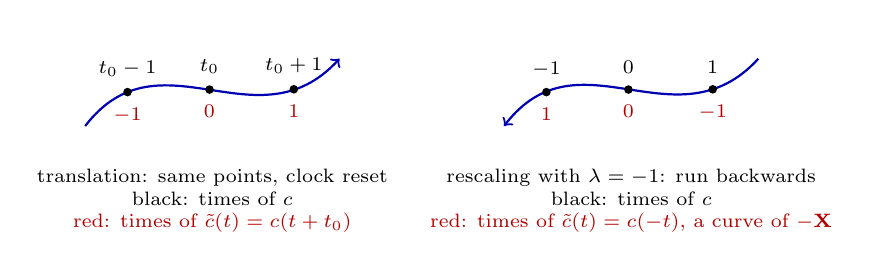
\begin{tikzpicture}[scale=0.95]
\draw[thick, blue!70!black, ->] (0,0) .. controls (1,1.3) and (2.3,-0.3) .. (3.4,0.9)
  node[pos=0.18, circle, fill=black, inner sep=1.1pt, label={[font=\scriptsize, text=black]above:$t_0 - 1$}, label={[font=\scriptsize, red!70!black]below:$-1$}] {}
  node[pos=0.5, circle, fill=black, inner sep=1.1pt, label={[font=\scriptsize, text=black]above:$t_0$}, label={[font=\scriptsize, red!70!black]below:$0$}] {}
  node[pos=0.82, circle, fill=black, inner sep=1.1pt, label={[font=\scriptsize, text=black]above:$t_0 + 1$}, label={[font=\scriptsize, red!70!black]below:$1$}] {};
\node[font=\scriptsize, align=center] at (1.7,-1.0) {translation: same points, clock reset\\ black: times of $c$\\ \textcolor{red!70!black}{red: times of $\tilde c(t) = c(t + t_0)$}};
\begin{scope}[xshift=5.6cm]
\draw[thick, blue!70!black, <-] (0,0) .. controls (1,1.3) and (2.3,-0.3) .. (3.4,0.9)
  node[pos=0.18, circle, fill=black, inner sep=1.1pt, label={[font=\scriptsize, text=black]above:$-1$}, label={[font=\scriptsize, red!70!black]below:$1$}] {}
  node[pos=0.5, circle, fill=black, inner sep=1.1pt, label={[font=\scriptsize, text=black]above:$0$}, label={[font=\scriptsize, red!70!black]below:$0$}] {}
  node[pos=0.82, circle, fill=black, inner sep=1.1pt, label={[font=\scriptsize, text=black]above:$1$}, label={[font=\scriptsize, red!70!black]below:$-1$}] {};
\node[font=\scriptsize, align=center] at (1.7,-1.0) {rescaling with $\lambda = -1$: run backwards\\ black: times of $c$\\ \textcolor{red!70!black}{red: times of $\tilde c(t) = c(-t)$, a curve of $-\mathbf{X}$}};
\end{scope}
\end{tikzpicture}
